\documentclass[12pt]{amsart}
\usepackage{graphicx, framed}
\usepackage{comment}
\usepackage{amscd}
\usepackage{amssymb,xcolor}
\usepackage[all, knot]{xy}
%\usepackage[top=1.2in, bottom=1.2in, left=1.2in, right=1.2in]{geometry}
\xyoption{all}
\xyoption{arc}
\usepackage{hyperref}



\renewcommand\labelitemii{$\diamondsuit$}


% The following causes equations to be numbered within sections
\numberwithin{equation}{section}


\theoremstyle{plain} %% This is the default, anyway
\newtheorem{thm}[equation]{Theorem}
\newtheorem{preproof}{Preproof Discussion}
\newtheorem{obs}{Observation}
\newtheorem{thmdef}[equation]{TheoremDefinition}
\newtheorem{introthm}{Theorem}
\newtheorem{introcor}[introthm]{Corollary}
\newtheorem*{introthm*}{Theorem}
%\newtheorem{question}{Question}
\newtheorem*{question}{Question}
\newtheorem{cor}[equation]{Corollary}
\newtheorem{lem}[equation]{Lemma}
\newtheorem{prop}[equation]{Proposition}
\newtheorem{porism}[equation]{Porism}
\newtheorem{algorithm}[equation]{Algorithm}
\newtheorem{axiom}[equation]{Axiom}
\newtheorem*{axioms*}{Axioms}
\newtheorem*{axiom*}{Axiom}
\newtheorem{conj}[equation]{Conjecture}
\newtheorem{quest}[equation]{Question}

\newcommand{\Aug}[1]{\section{August #1, 2022}}
\newcommand{\Sept}[1]{\section{September #1, 2022}}
\newcommand{\Oct}[1]{\section{October #1, 2022}}
\newcommand{\Nov}[1]{\section{November #1, 2022}}
\newcommand{\Dec}[1]{\section{December #1, 2022}}

\newcommand{\rsa}{\rightsquigarrow}


\theoremstyle{definition}
\newtheorem{defn}[equation]{Definition}
\newtheorem{chunk}[equation]{}
\newtheorem{ex}[equation]{Example}

\newtheorem{exer}[equation]{Exercise}

\theoremstyle{remark}
\newtheorem{rem}[equation]{Remark}

\newtheorem{notation}[equation]{Notation}
\newtheorem{terminology}[equation]{Terminology}

%%%%%%%%%%%%%
% local definitions
%%%%%%%%%%%%%


\newcommand{\R}{\mathbb{R}}

\makeindex

\begin{document}


\setcounter{tocdepth}{1}
\tableofcontents


\Aug{23}

This class is, as its name makes clear, is all about differential equations. Let's start with an example that is probably similar to something you've seen in Calculus.

\begin{ex}
The equation
\[ \frac{dy}{dx} = 7 y\]
is a differential equation. The unknown in this equation, $y$, stands for a function. What makes this equation a differential equation is that the equation relates the mystery function and its derivative.

Let's see if we can guess a solution. This equation might remind us of a curious calculus coincidence. If the $7$ wasn't there, we would be looking for a function whose derivative is equal to itself; $e^x$ would work. 

Let's try $y=7e^x$ for our original equation. To test it, we plug it in:
\[ y = 7 e^x \rsa y' = (7e^x)' = 7e^x \neq 7y = 49e^x.\]
How about putting the $7$ somewhere else:
\[  y = e^{7x} \rsa y' = (e^{7x})' = e^{7x} (7x)' = 7 e^{7x} = 7y.\]
So $e^{7x}$ is a solution!

Could there be any others?
\[  y = 5e^{7x} \rsa y' = (5e^{7x})' = 5e^{7x} (7x)' = 7 (5e^{7x}) = 7y.\]

In general, $y(x) = C e^{7x}$ is a solution for any constant $C$.
\end{ex}

Of course, at the end of the day, nothing was special about $7$. If we replaced $7$ by any real number $a$, for the same reason, we would find that for the differential equation
\[ y' = ay\]\index{$y'=ay$}
the \emph{general solution}\index{general solution} is
\[ y(x) = C e^{ax}.\]

Guessing, while successful here, is not going to be our preferred method in the class. Let's savor this victory, and be prepared to collect many methods for solving differential equations as we progress through the course.

\subsection*{Types of differential equations (\S1.1)}
There are many different ways of throwing together functions and derivatives in an equation, so we'll need some terminology to orient ourselves.

\begin{defn} An \emph{ordinary differential equation (ODE)}\index{ordinary differential equation}\index{ODE} is a differential equation involving only one independent variable; i.e., derivatives with respect to just one variable.
\end{defn}
 For example,
 \[ \frac{d^2 y}{dt^2} + t \frac{dy}{dt} = -y + \cos(ty)\]
 is an ordinary differential equation.
 
In general an ODE is an equation of the form \[F(t,y,y',y'',\dots,y^{(n)})=0\] for some function $F$ where $y=y(t)$: an equation relating the function $y$ with its derivative(s).

\begin{defn} A \emph{partial differential equation (PDE)}\index{partial differential equation}\index{PDE} is a differential equation involving multiple independent variable; i.e., derivatives with respect to different variables.
\end{defn}
For example, 
\[ \frac{\partial u}{\partial t} - 5 \frac{\partial u}{\partial x} = 0\]
and 
\[ \frac{\partial^2 z}{\partial x \partial y} -z^2 = xy\]
are PDEs. A solution of the first PDE would be a function $u(x,t)$ that depends two independent variables $x$ and $t$.
 
The ``ordinary'' vs ``partial'' refers to what type of derivatives see. 

This is a class about ODEs. Almost all of the rest of the differential equations we see this semester will be ordinary!


\begin{defn} The \emph{order}\index{order} of a differential equation is the highest order derivative that occurs in the equation.
\end{defn}

For example,
\[ y y'' +  y''' + \frac{1}{y} = 5x\]
is a third order ODE, due to the $y'''$ term and
 \[ \frac{d^2 y}{dt^2} + t \frac{dy}{dt} = -y + \cos(ty)\]
 is a second order ODE.
 
 \begin{defn} A \emph{linear}\index{linear} ODE is any ODE of the form
 \[ a_n(t) y^{(n)} + a_{n-1}(t) y^{(n-1)} + \cdots + a_2(t) y'' + a_1(t) y' + a_0(t) y = f(t).\]
 \end{defn}
 For example,
 \[ 5t y'' + \ln(t) y' + y = \cos(t)\]
 is a second order linear ODE, but 
 \[ y y' + 5y = 7\]
 and 
 \[ (y')^3 - t y^2 = 3 e^t\]
are first order nonlinear ODEs.

We will be especially interested in linear ODEs in this course!

 
\subsection*{Discussion Questions}
\begin{enumerate}
\item Is the differential equation $y' = y^{2/3}$ ordinary? linear? What is its order?
\begin{framed}
Ordinary yes, linear no, order 1.
\end{framed}
\item Which of the following is a solution to the differential equation $y' =y^{2/3}$:
\begin{enumerate}
\item $y=8 t^2$
\item $y= e^{{2t/3}}$
\item $y=\frac{1}{27} t^3$
\item $y=0$ (constant function 0)
\end{enumerate}
\begin{framed}
\begin{enumerate}
\item No: $y' = 16t \neq y^{2/3} = 4t^{4/3}$.
\item No: $y' = 2/3 e^{2t/3} \neq y^{2/3} = (e^{2t/3})^{2/3} = e^{4t/9}$.
\item Yes: $y' = \frac{1}{9} t^2 = y^{2/3}$.
\item Yes: $y'=0=y^{2/3}$.
\end{enumerate}
\end{framed}
\item There is a solution to $x y'' = (4x -4) y$ of the form $y=xe^{ax}$ for some real number $a$. Find $a$.
\begin{framed}
By the product rule, \[y'=(ax+1) e^{ax} \quad \text{and} \quad y''=(a^2 x + 2a) e^{ax},\] so  \[xy'' - (4x-4)y = (a^2 x^2 +2ax) e^{ax} - (4x-4)x e^{ax}.\] If this is zero, we must have \[a^2 x^2 + 2ax = 4x^2 - 4x\] as functions of $x$, so $a=-2$.
\end{framed}
\item[(4*)] If $f,g$ are solutions to $y^{(3)} + 2e^x y^{(2)} -y = \cos(x)$, show that $\frac{f+g}{2}$ is too.
\item[(5*)] Using only calculus, justify the claim we made earlier that $y=Ce^{ax}$ is the general solution to $y'=ay$ for any $a\in \R$. That is, explain why there aren't any other solutions (exponential or otherwise).
\end{enumerate}

\subsection*{Initial value problems}

In our first example, we saw that there are many solutions to the differential equation $y'=7y$. To pin one down, we might specify a value for our function at a point. The system
\[\begin{cases} y' = 7y \\ 
y(2)=4 \end{cases}\]
is a example of an \emph{initial value problem (IVP)}\index{initial value problem}\index{IVP}. Geometrically, $y(2)=4$ corresponds to the condition that the graph of our solution passes through $(2,4)$.




\Aug{25}

\begin{ex}\label{ex:first IVP}
\[\begin{cases} y' = 7y \\ 
y(2)=4 \end{cases}\]
is a example of an \emph{initial value problem}. Geometrically, $y(2)=4$ corresponds to the condition that the graph of our solution passes through $(2,4)$.


We can solve this using our solution of $y'=7y$ from earlier. We have
\[ y= Ce^{7x} \qquad y(2)=4\]
so \[ 4 = C e^{7 \cdot 2}\]
and \[ C= 4e^{-14}.\]
That is,
\[ y= 4e^{-14}e^{7x} = 4 e^{7x-14}.\]
\end{ex}

\subsection*{Modeling with differential equations (\S1.3)}

Differential equations is one of the most useful areas of math for applications, since so many real life things are described effectively by differential equations. A \emph{mathematical model}\index{mathematical model} is a description of some system or phenomenon by an equation or a formula. A model is rarely perfect, since we can't even know all of the factors that might affect something, but we can often use them to understand things better.

Let's start with a basic example.

\begin{ex} \index{population model}A classical model of human population growth is based on the assumption that the rate at which the population of a country grows is proportional to the population of that country. To express this as a differential equation, let $P$ the population of a country. We are interested in how it changes, so let $t$ be a variable for time and view $P$ as a function of $t$.  To say that two things are \emph{proportional}\index{proportional} means that the exists a constant $k$ (called the \emph{constant of proportionality}) such that $k$ times the first quantity is the second quantity. The rate of change of the population is $\frac{dP}{dt}$. Thus, our equation is
\[ \frac{dP}{dt} = kP \]
for some constant $k$. We do not know what $k$ is without further information.

This is the only differential equation we've solved! We must have 
\[ P(t) = C e^{kt}.\]
Given two data points for any specific population, we can determine $C$ and $k$.
\end{ex}



Let us try to set up a more complicated model.

\begin{ex} \index{mixing model}Say that we have a tank of water. At first, it holds $500$ liters of pure water (no salt). After  switch is flipped, salt water that has 7 grams of salt per liter starts flowing in at a rate of 2 liters per minute, and water from the bottom of the tank starts flowing out at a rate of 2 liters per minute. 
%We assume that the water stays well mixed so that the water flowing out is as salty as the average water in the tank. 
Let's model the amount of salt in the tank at a given time after the switch is flipped.

Let $A$ be the amount of salt in the tank, in grams, and $t$ be the amount of time since the switch is flipped in minutes.
We need to understand the rate of change of $A$. Salt enters at a rate of $7 \cdot 2 = 14$ grams per minute. To find the rate at which salt exits, the amount of salt in an average liter of water is $A/500$ grams per liter, so the amount of salt exiting is $2 \cdot A/500 = A/250$.

We obtain the differential equation
\[ \frac{dA}{dt} = 14 - \frac{A}{250}.\]
We also have the initial condition $A(0)=0$.

We will learn how to solve systems like this soon.
\end{ex}







\subsection*{Discussion Questions}

\index{counterfeit money}
The government of a country wants to remove counterfeit money from circulation. Say there are 20 million total bills in circulation. Every day, 4 million of its bills pass though federal banks, and every counterfeit bill collected is replaced by a legal one. Say that half of the total bills in circulation today are counterfeit. Let's assume that the total number of bills in circulation stays constant and that no more counterfeit bills are being introduced. Our goal is to find an initial value problem modeling the percentage of counterfeit bills in circulation as time passes. 

\begin{enumerate}
\item Introduce variables to keep track of the quantities we are interested in. What is the independent variable and what is the dependent variable? What are the units for each?
\item To set up a differential equation, we want to relate the dependent variable with its rate of change. On average, what is the change in the number of counterfeit bills each day\footnote{Hint: First figure out how many counterfeit bills pass through federal banks each day, on average.}?
\item Express the previous part as a differential equation.
\item We also need an initial condition. Write it down.
\item This is a type of differential equation we've solved already. Find an explicit solution.
\item Based on your model, when will the total number of counterfeit bills pass below 3 million?
\end{enumerate}
\begin{framed}
\begin{enumerate}
\item Take $t$ for time (number of days after today), and $C$ to be the number of millions of counterfeit bills in circulation. $C$ is dependent on $t$.
\item First the number of bills that pass through banks on an average day is $4C/20 = C/5$: the proportion of counterfeit bills times the total number of millions of bills passing through the banks. Thus, $C$ decreases by $C/5$ on average each day.
\item $C'=-C/5$.
\item $C(0)=10$.
\item $C(t)=ke^{-t/5}$ is the general solution. We plug in $C(0)=10$ to get $k=10$, so $C(t)=10 e^{-t/5}$.
\item $C(t)=3$ gives us $10e^{-t/5}=3$. Then $t=-5 \ln(3/10) \approx 6$. It should take about $6$ days.
\end{enumerate}
\end{framed}

Let's do an experiment to test our model. Each coin you've been given represents a million bills. Some represent valid coins and some represent counterfeits. Every day, take four random coins; replace the counterfeits with legal ones, and leave the legal ones alone.

\begin{enumerate}
\item Discuss whether your model for the previous situation is relevant to this experiment. What aspects fit the story well, and what ones don't?
\item Run the experiment, keeping track of the number of counterfeit bills each day, and how long it takes to get down to 3 counterfeits. Even better, run the experiment a few times.
\end{enumerate}

Now let's change our original story. As before, every day, 4 million of its bills pass though federal banks, and every counterfeit bill collected is replaced by a legal one. Say that half of the 20 million total bills in circulation today are counterfeit. But now, let's assume that 1 million new legal bills and 1 million new counterfeit bills are put into circulation each day.

\begin{enumerate}
\item Create a new differential equation and initial value problem to model this situation\footnote{Hint: You might find it helpful to write a closed formula for the number of total bills in circulation at a given time first.}. 
%You might find it helpful to write a closed formula for the number of total bills in circulation at a given time first.
%\item This is not a differential equation that we have solved yet. We will learn how to find explicit solutions of equations like this soon! But even without knowing what exactly the solution is, explain why there is one and only one solution to this initial value problem.
\item Run an experiment similar to the one above adapted to this situation.
\item Based on the experiment, what do we expect to happen to the currency as time passes?
\end{enumerate}
\begin{framed}
\begin{enumerate}
\item Let's use $t$ and $C$ as names again. The total number of bills at time $t$ is now $20+2t$. Now $C'(t) = 1 - \frac{4 C}{20+2t} = 1-\frac{2C}{10+t}$, and $C(0)=10$ again.
\end{enumerate}
\end{framed}

\begin{comment}

\Aug{30}

We will now spend a while focusing on first-order ODEs and corresponding initial value problems: all of Section 1.2 and Chapter 2 will be about this setting.

\subsection*{Existence and uniqueness for initial value problems (\S1.2)}
If our goal in solving an initial value problem
\[\begin{cases} y' = f(x,y) \\ y(x_0) = y_0\end{cases}\]
 is to find \emph{the} function that satisfies the two conditions, for this goal to make sense, there should be a function, and only one function that satisfies the two conditions. The \emph{existence}\index{existence} question for an IVP is whether there is any function that satisfies both conditions; the \emph{uniqueness}\index{uniqueness} question for an IVP is whether there is at most function that satisfies both conditions. (Actually \emph{finding} this function is a different question.)

Let's consider these things in some examples we have seen before.

\begin{ex} In Example~\ref{ex:first IVP}, we considered the IVP
\[\begin{cases} y' = 7y \\ 
y(2)=4 \end{cases}\]
and saw that the function $y= 4 e^{7x-14}$ was the one and only solution. Thus, there exists a unique solution in this case.
\end{ex}


On the other hand, we have the following.

\begin{ex} Consider the IVP
\[\begin{cases} y' = y^{2/3} \\ 
y(0)=0 \end{cases}.\]
We saw in the Discussion Questions from Aug 25 that $y=0$ and $y=\frac{1}{27} t^3$ both satisfy the first differential equation. Both of these functions also satisfy the initial condition, so they are also both solutions to the IVP. Here we have an IVP for which the solution is not unique.
\end{ex}

We can even have no solution sometimes.

\begin{ex} Consider the IVP
\[\begin{cases} y' = \begin{cases} 1 & \text{if } y\geq 0 \\ -1 & \text{if } y  <0\end{cases}\\ y(0) = 0\end{cases}.\]
This IVP has no solution! (You can convince yourself why not.)
\end{ex}

Luckily, there is a theorem that guarantees existence and uniqueness of solutions IVP's under certain hypotheses.

\begin{thm}[Picard-Lindel\"of]\index{Picard-Lindel\"of} For the IVP
\[\begin{cases} \frac{dy}{dx} = f(x,y) \\ 
y(x_0) = y_0 \end{cases}\]
and some rectangle $R$ in the $(x,y)$-plane containing $(x_0,y_0)$ in its interior,
there exists a unique solution on some possibly smaller interval $(x_0 - h, x_0+h)$, so long as $f$ and $\frac{\partial f}{\partial y}$ are continuous on $R$.
\end{thm} 

\begin{ex} Consider the differential equation
\[ \frac{dy}{dx} = 5 xy.\]
We want to use the Picard-Lindel\"of Theorem to show that for any initial condition $y(x_0)=y_0$, there is a unique solution near $x_0$. The $f(x,y)$ of the Theorem is $5xy$; this is continuous on all of $\mathbb{R}^2$. We also need to look at $\frac{\partial f}{\partial y} = 5x$. This is also continuous on all of $\mathbb{R}^2$.
We conclude that 
\[\begin{cases} \frac{dy}{dx} = 5xy \\ 
y(x_0) = y_0 \end{cases}\]
has a unique solution, no matter what $x_0$ and $y_0$ are.
\end{ex}

\begin{ex} Let's consider
\[\begin{cases} y' = y^{2/3} \\ 
y(x_0) = y_0 \end{cases}.\]
Here $f(x,y) = y^{2/3}$ and $\frac{\partial f}{\partial y}(x,y) = \frac23 y^{-1/3}$. $f$ is continuous everywhere, but $f'$ is only continuous where $y_0\neq 0$.
Thus, if $y_0\neq 0$, then there is a unique solution.

However, if $y_0=0$, the theorem does not apply. We looked at this example earlier and saw that the solutions were not unique for $(x_0,y_0) = (0,0)$.
\end{ex}


\begin{ex} Let's consider
\[ \begin{cases} y' = \frac{y^2}{t^2-4} \\
y(-1) = 3 \end{cases}.\]
What is the largest interval on which the Picard-Lindel\"of Theorem guarantees the existence of a unique solution?
We have, in the notation of the Theorem,
\[ f = \frac{y^2}{t^2-4} \qquad \frac{\partial f}{\partial y}=\frac{2y}{t^2-4}.\]
These are continuous except when $t=\pm 2$. Thus, any rectangle whose base is contained in $(-2,2)$ will satisfy the hypotheses of the theorem, so $(-2,2)$ is the interval we seek.
\end{ex}

\subsection*{Solution curves from slope fields (\S 2.1)} There is a great way to visualize solutions to differential equations without solving them. The idea is to think of $\frac{dy}{dt}$ geometrically as the slope of the graph of $y$.

\begin{ex}\label{ex:first aut} Consider the differential equation 
\[ y' = 3-y.\]
We won't try to write down a solution yet. Instead, on the plane, we draw little lines with slope $3-y$ at various points.\\
\begin{center}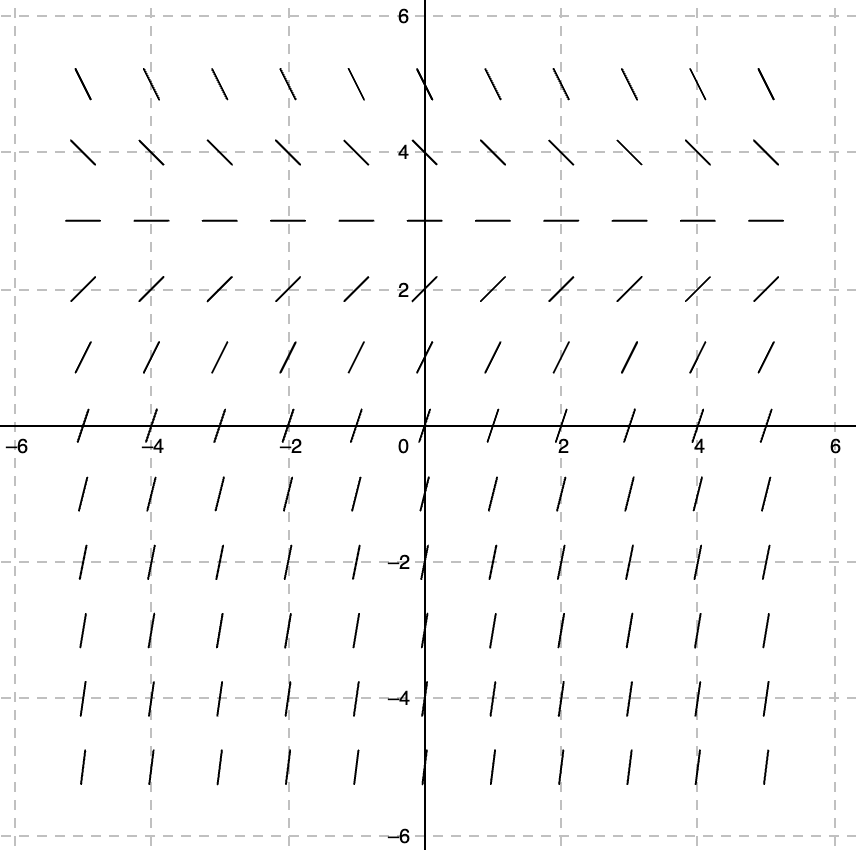
\includegraphics[scale=.5]{sf1}\end{center}
We can use this to sketch the solution to the IVP
\[\begin{cases} y' = 3-y \\
y(2)= 2 \end{cases}\]
by starting at $(2,2)$ and going along with the flow.
\begin{center}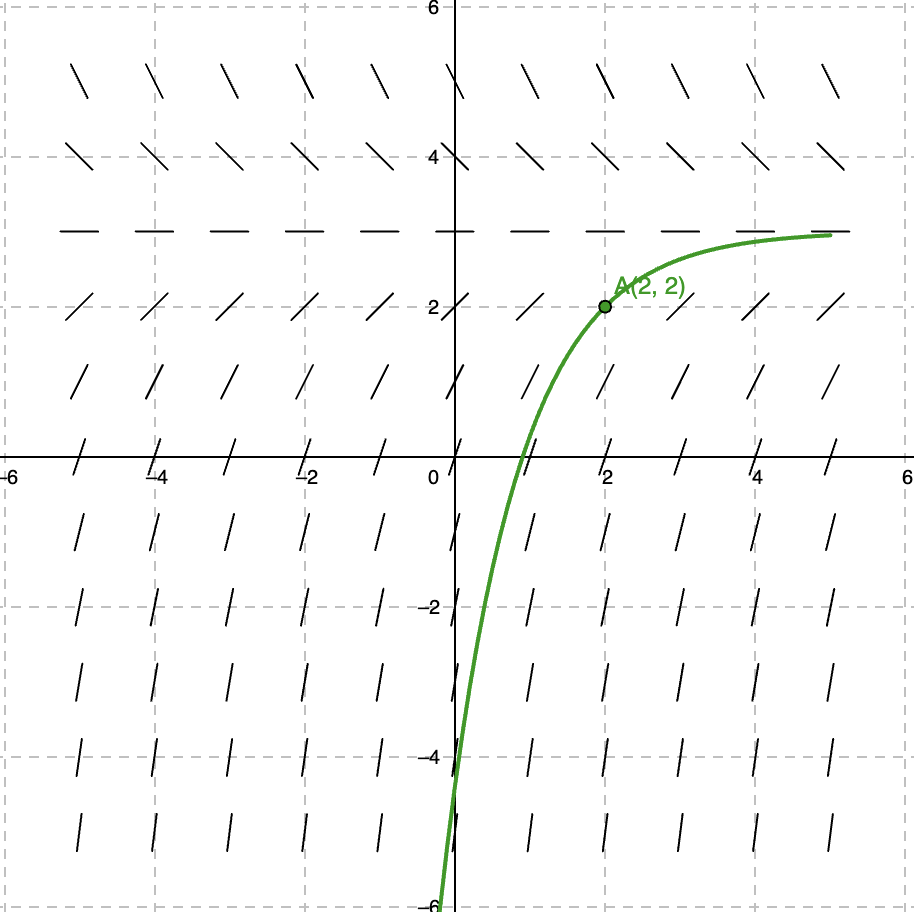
\includegraphics[scale=.5]{sf2}\end{center}

Or 
\[\begin{cases} y' = 3-y \\
y(-4)= 4 \end{cases}:\]
\begin{center}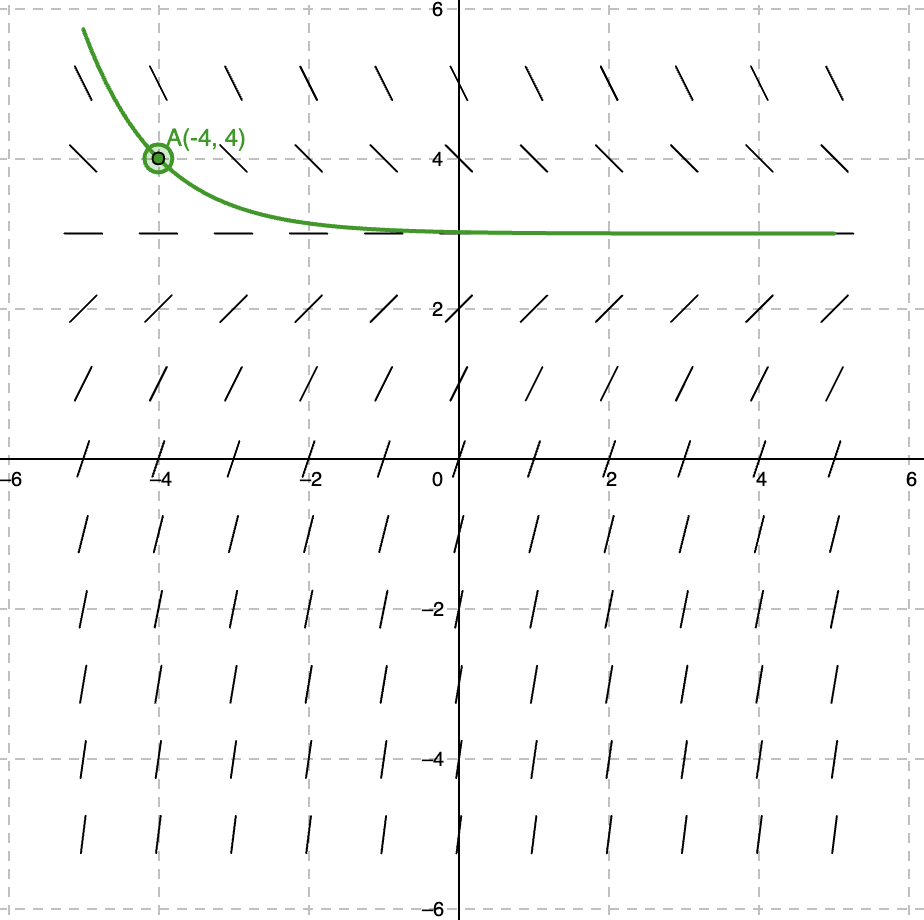
\includegraphics[scale=.5]{sf3}\end{center}
\end{ex}

The picture we drew above is called a \emph{slope field}.\index{slope field}

\subsection*{Discussion Questions} Draw a slope field for the differential equation
\[ y'= x+y\] and use it to sketch the solutions with initial conditions
\begin{enumerate}
\item $(0,1)$
\item $(0,0)$
\item $(0,-1)$
\item $(0,-2)$
\end{enumerate}
\begin{framed}
\begin{center}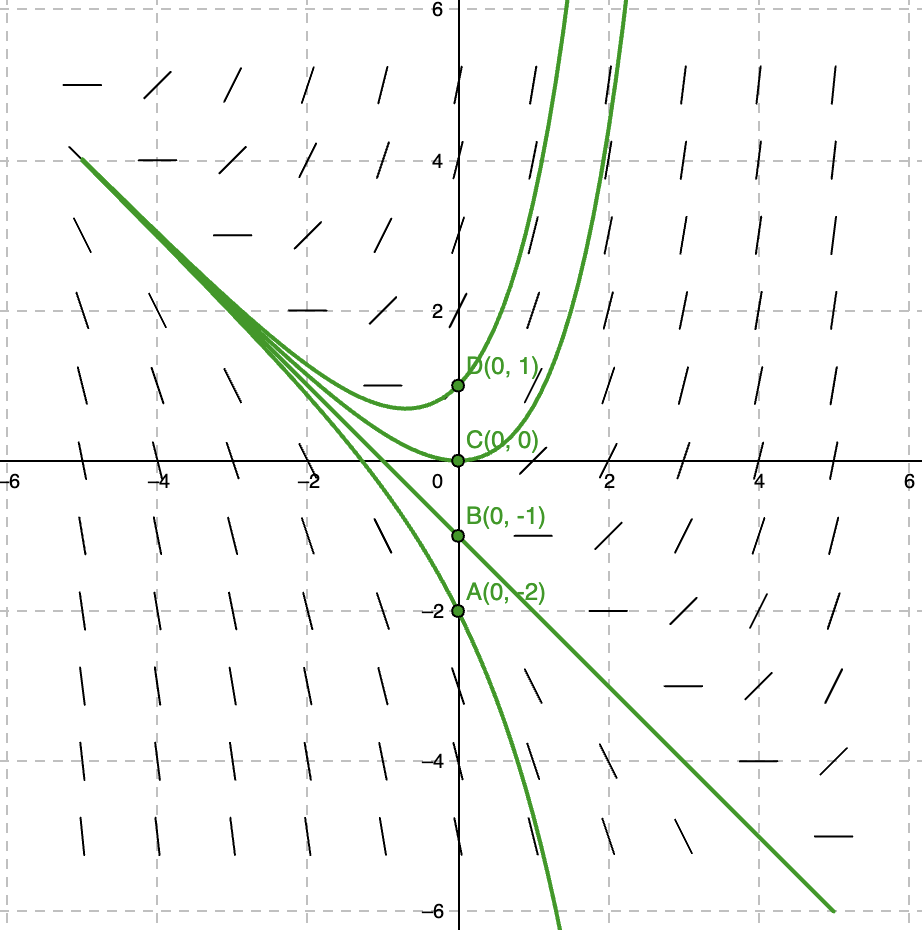
\includegraphics[scale=.5]{sf4}\end{center}
\end{framed}

\subsection*{Autonomous differential equations}
Example~\ref{ex:first aut} belongs to a class of equations that is worth singling out.
\begin{defn} A differential equation of the form \[ y' = f(y)\]
 is said to be \emph{autonomous}.\index{autonomous}
 \end{defn}
 
 The behavior of a solution of an autonomous differential equation is determined entirely by the current value of the function (and not the independent variable).
 
For an autonomous differential equation, whether a solution is increasing, decreasing, or constant at a point only depends on the $y$-value at that point. We can determine this either algebraically or using the slope field.

\begin{ex}
Consider the autonomous differential equation 
\[ y' = \frac{y^3}{9} -y.\]
A solution to this equation will be increasing when $y'>0$, which is the same as $\frac{y^3}{9} -y>0$. This happens when $y\in (-3,0)\cup (3, \infty)$.
A solution to this equation will be decreasing when $y'<0$, which is the same as $\frac{y^3}{9} -y<0$. This happens when $y\in (0,3)\cup (-\infty,-3)$.
A solution to this equation will be constant when $y'=0$, which is the same as $\frac{y^3}{9} -y=0$. This happens when $y=-3,0,3$.
We can also use the slope field to determine when it is increasing or decreasing.
\begin{center}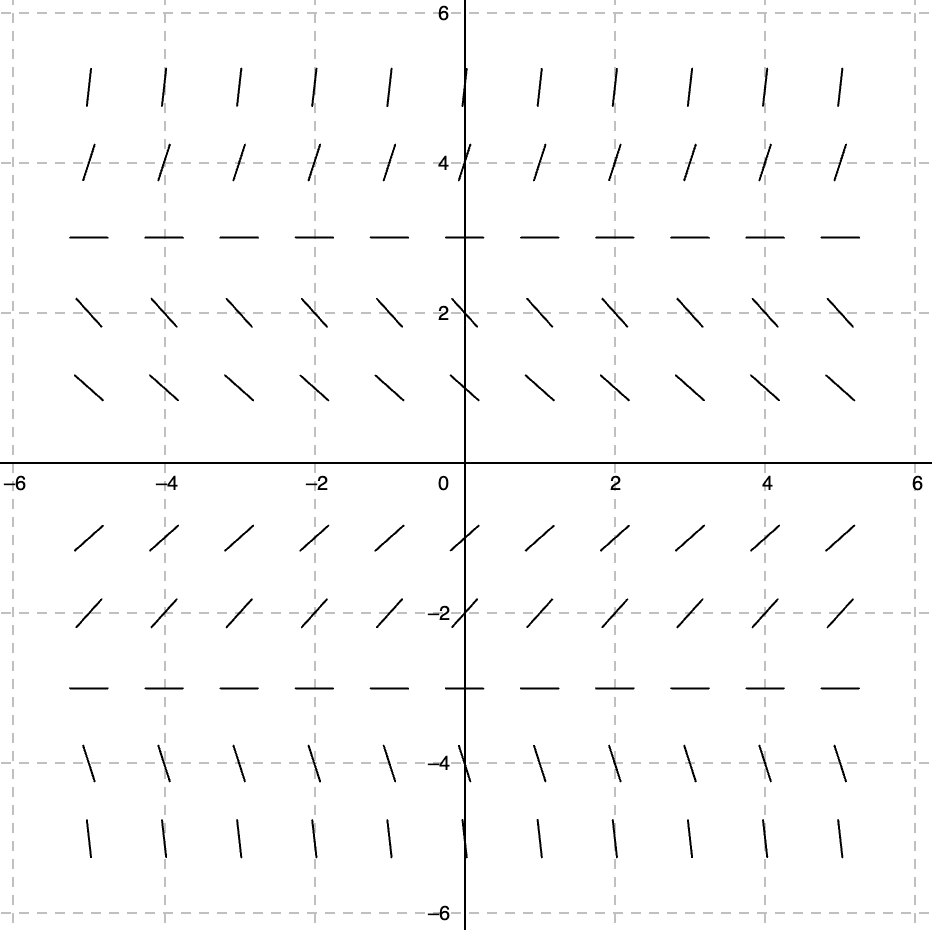
\includegraphics[scale=.5]{sf5}\end{center}
Let's sketch some solutions:
\begin{center}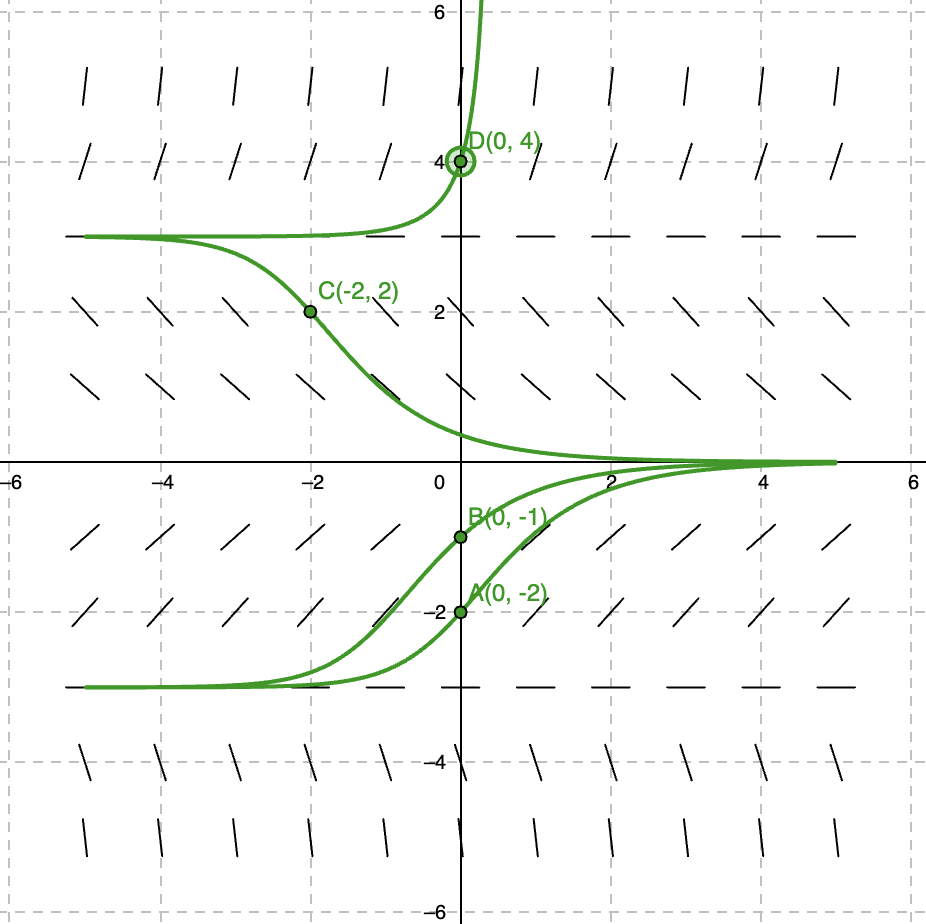
\includegraphics[scale=.5]{sf6}\end{center}
\end{ex}

A constant solution to an autonomous differential equation is also called an \emph{equilibrium solution}\index{equilibrium solution}.


\subsection*{Review of integration} Now we will start to collect some techniques for solving differential equations. Of course integration will play a big role. Let's review some basic techniques of integration. We will usually be using \emph{indefinite integration} or \emph{antidifferentiation} in this class. First, let's recall a list of building block functions whose integrals we need to know. 

\begin{itemize}
\item $\int x^n \, dx = \frac{x^{n+1}}{n+1} + C$ when $n\neq -1$.
\item $\int \frac{1}{x} \, dx = \ln(x) + C$.
\item $\int e^x \, dx = e^x + C$.
\item $\int \sin(x) \, dx = -\cos(x) + C$.
\item $\int \cos(x) \, dx = \sin(x) + C$.
\end{itemize}

We also have many rule for how to integrate complicated functions in terms of integrating smaller parts. There are two easy rules to get us started.

\begin{itemize}
\item $\int f(x) + g(x) \, dx = \int f(x)  \, dx + \int g(x) \, dx$.
\item $ \int c f(x) \, dx = c \int f(x)  \, dx$ for any constant $c$.
\end{itemize}

Unlike with derivatives, there is no direct rule for computing the integral of a composition or a product. Instead, we have ``$u$-substitutions''\index{u-substitution} and ``integration by parts''\index{integration by parts}. 

$u$-substitution is a technique that is likely to work when we can see some function and something like its derivative inside the function we are trying to integrate. In this case, we set the function to be $u$, we set $du= u'(x) \, dx$, and we try to rewrite our integrand as some function of $u$  times $du$ (and get rid of our starting variable entirely). $u$-substitutions also work well when instead of some function of $x$, we have a function of $x-a$ or a function of $ax$ for some constant $a$.
This is the main technique that we will want to use, other than the basic rules.


examples


Integration by parts is a technique that might work when our integrand is a product of two things, one of which we know how to integrate (i.e., looks like the derivative of something). The general rule is if we can find functions $u(x), v(x)$ such that our integral is $\int u \, dv$ (where $dv = v'(x) \, dx$), the we have
\[ \int  u \, dv = uv -  \int v \, du;\]
and if we can integrate $ \int v \, du$, we are done. A rule of thumb for what to choose for $u$ vs what to choose for $dv$ in integration by parts is LIATE (log, inverse trig, algebraic, trig, exponential): stuff on the left is usually better for $u$'s and stuff on the right is usually better for $dv$'s.

examples.

\subsection*{Separable first-order equations (\S2.2)}






\begin{comment}
\end{comment}

\printindex

\end{document}













 